\documentclass[../../main.tex]{subfiles}
\graphicspath{{\subfix{../../image/}}} % 指定图片目录,后续可以直接使用图片文件名。

% 例如:
% \begin{figure}[h]
% \centering
% \includegraphics{image-01.01}
% \caption{图片标题}
% \label{fig:image-01.01}
% \end{figure}
% 注意:上述\label{}一定要放在\caption{}之后,否则引用图片序号会只会显示??.

\begin{document}

\section{主理想整环与唯一分解整环}

\begin{definition}[主理想整环]
设 $(R, +, \cdot)$ 是一个交换环,则我们称 $R$ 是个\textbf{主理想整环},若 $R$ 是一个整环,而且每一个理想 $I \lhd R$ 都是主理想,即可以写成
\begin{align*}
I = (a) = Ra
\end{align*}
的形式。
\end{definition}

\begin{proposition}
$(\mathbb{Z}, +, \cdot)$ 是个主理想整环。
\end{proposition}
\begin{proof}

\end{proof}

\begin{lemma}
$(\mathbb{Z}, +, \cdot)$ 的每个子群都具有 $n\mathbb{Z}$ 的形式。
\end{lemma}
\begin{proof}
不妨令 $I < \mathbb{Z}$ 是加法子群。

假如 $I$ 只包含了 $0$ 一个元素,那么 $I = \{0\} = 0\mathbb{Z}$。

假设 $I$ 包含了 $0$ 以外的元素,那么根据逆元的封闭性,$I$ 一定包含了一个正整数。根据自然数集的良序公理,我们可以取到最小的那个正整数,称其为 $n$。下面,我们只须证明
\begin{align*}
I = n\mathbb{Z}
\end{align*}
一方面,因为 $n \in I$,则 $n$ 生成的(加法)子群也包含于 $I$,而前者正是 $n\mathbb{Z}$,因此
\begin{align*}
n\mathbb{Z} \subset I
\end{align*}
另一方面,假设存在 $I \setminus n\mathbb{Z}$ 的元素,我们任取 $m \in I \setminus n\mathbb{Z}$。则根据带余除法,我们有
\begin{align*}
m = qn + r
\end{align*}
其中 $1 \leqslant r \leqslant n - 1$。

则根据子群的性质,
\begin{align*}
r = m - qn = m + (-q)n \in I
\end{align*}
而这与 $n$ 是 $I$ 最小的正整数的事实相矛盾。这就证明了这个引理,进而证明了上面的命题,即 $(\mathbb{Z}, +, \cdot)$ 是个主理想整环。 
\end{proof}

\begin{proposition}
若 $(R, +, \cdot)$ 是一个域,则 $R$ 是一个主理想整环。
\end{proposition}
\begin{proof}

\end{proof}

\begin{lemma}
若 $(R, +, \cdot)$ 是一个环,则 $R$ 是一个域当且仅当 $\{0\}$ 和 $R$ 是 $R$ 中唯二的理想 $(R \neq \{0\})$。
\end{lemma}
\begin{proof}
先证充分性。假设 $R$ 是一个域,而 $I$ 是一个理想。假设 $I \neq \{0\}$,任取 $a \neq 0$。则存在 $b \in R$,使得
\begin{align*}
ab = 1
\end{align*}
因此
\begin{align*}
1 \in Ra \subset RI \subset I
\end{align*}
所以 $I = R$。

再证必要性。假设 $R$ 唯二的理想是零和整个环。令 $a \neq 0$,则 $(a) \neq 0$,因此 $(a) = R$。于是存在 $b, c \in R$,使得
\begin{align*}
ab = 1 \in R\\
ca = 1
\end{align*}
下面我们只须证明 $b = c$,而证明方法和我们当时证明逆元是唯一时是一样的。
\begin{align*}
b = 1b = cab = c1 = c
\end{align*}
这样,就证明了 $R$ 是一个域。
\end{proof}

\begin{proposition}
设 $(R, +, \cdot)$ 是一个主理想整环,而 $\mathfrak{p} \lhd R$ 是一个素理想且 $\mathfrak{p} \neq \{0\}$,则 $\mathfrak{p}$ 是一个极大理想。
\end{proposition}
\begin{proof}
用反证法。假设 $\mathfrak{p}$ 是素理想,而不是极大理想,则存在 $I \lhd R$,使得 $\mathfrak{p} \subsetneq I \neq R$。

因为 $R$ 是主理想整环,我们记 $\mathfrak{p} = (p)$,$I = (a)$。则由于 $\mathfrak{p} \subset I$,我们有
\begin{align*}
p \in I = (a)
\end{align*}
故存在 $b \in R$,使得
\begin{align*}
p = ab
\end{align*}
显然,$b$ 不能是单位(即存在乘法逆元的元素),因为不然的话我们就可以写 $a = pb^{-1}$,进而 $\mathfrak{p} = I$,导致矛盾。因此,$b$ 没有乘法逆元。

另外,由于 $I$ 是真理想,故 $a$ 也不是单位——否则 $1 \in (a)$,进而 $(a) = R$。

现在 $ab \in \mathfrak{p}$,则 $a \in \mathfrak{p}$ 或 $b \in \mathfrak{p}$。假如 $a \in \mathfrak{p} = (p)$,则不难证明 $b$ 就是一个单位,而这是不可能的。假如 $b \in \mathfrak{p}$,则同理,$a$ 就是一个单位,而这也是不可能的。无论如何,我们都会得到矛盾。

因此,我们就证明了,在主理想整环中,每一个素理想都是极大理想,因此两个概念在主理想整环中是等价的。 
\end{proof}

\begin{figure}[H]
\centering
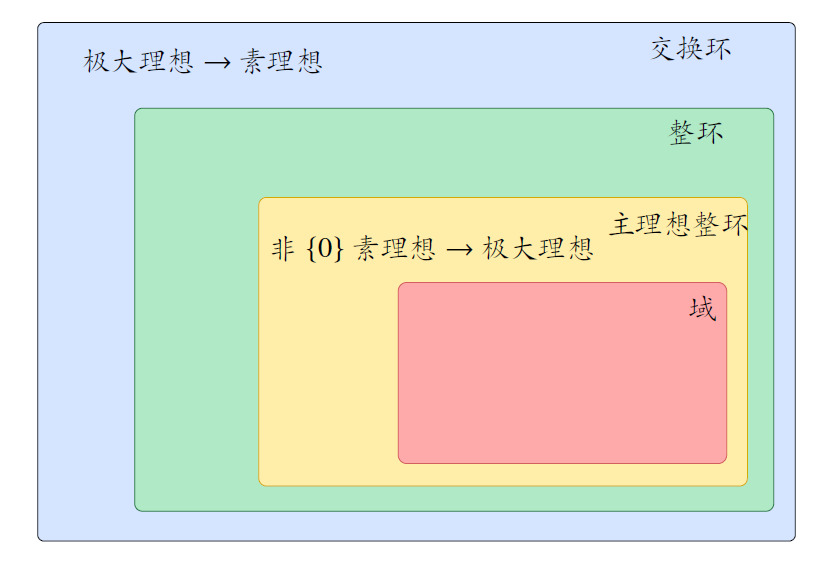
\includegraphics[scale=0.4]{环的层级关系以及素理想和极大理想之间的关系.png}
\caption{环的层级关系以及素理想和极大理想之间的关系}
\label{figure:环的层级关系以及素理想和极大理想之间的关系}
\end{figure}

\begin{proposition}
若 $p$ 是一个素数,则 $\mathbb{Z}_p$ 是一个域。
\end{proposition}
\begin{proof}

\end{proof}
**命题 2.32** 
\begin{proposition}
$\mathbb{Z}_p$ 是一个域。
\end{proposition}
\begin{proof}
我们知道 $p\mathbb{Z} \lhd \mathbb{Z}$ 是个素理想,而 $\mathbb{Z}$ 是个主理想整环,因此 $p\mathbb{Z}$ 是 $\mathbb{Z}$ 的极大理想。根据之前的引理,这就证明了 $\mathbb{Z}_p$ 是一个域。
\end{proof}

\begin{definition}
若 $p$ 是一个素数,则我们把 $\mathbb{Z}_p$ 记作 $\mathbb{F}_p$。特别地,这是一个有限域,即只有有限多个元素的域。
\end{definition}

\begin{lemma}
若 $n$ 是一个合数,则 $\mathbb{Z}_n$ 不是一个域。
\end{lemma}
\begin{proof}
证明是类似的,故留做练习。
\end{proof}





\end{document}